\section{Lecture 18: IIR Filter Design}
%
Recall that the infinite impulse response (IIR) is written
as some combination of input and previous output values,
%
\begin{displaymath}
  y[n] = \sum_{m=0}^M b[m]x[n-m] - \sum_{k=1}^N a[k]y[n-k] \,,
\end{displaymath}
%
where the first summation is simply a FIR filter, and the convolutional
sum between $a$ and $y$ begins at $k=1$ since we assume $a[0] = 1$,
the multiplier of $y[n]$ on the LHS. The transfer
function, as we have previously seen, is given by
%
\begin{displaymath}
  H(z) = \infsum{n}h[n]z^{-n}
  = \frac{\sum_{m=0}^M b[m]z^{-m}}{\sum_{n=0}^N a[n]a^{-n}}
  = \frac{B(z)}{A(z)} \,.
\end{displaymath}
%
There are several differences with FIR filters:
%
\begin{enumerate}
\item IIR filters do not have linear phase; a linear phase
  was obtained as a result of the symmetry of the impulse response,
  but since this is of infinite duration for an IIR filter, there
  is no central point about which the impulse response can be
  symmetric since we require that the filter be causal.
\item IIR filters have low orders relative to their FIR counterparts,
  and are sufficient to implement ``tight'' filter specifications, e.g.
  very steep dropoff in the transition region.
\item We typically start by designing an analog filter, then convert
  this to digital.
\end{enumerate}
%
The design process for an IIR filter is broadly the same as that for
and FIR filter; we begin by selecting some desired frequency
response, $H_\mathrm{des}(\omega)$, then choose the class of filter we'd like
to use (e.g. IIR filter of order $N$ in both numerator and
denominator). A distance measure, or error, is then chosen between
$H(\omega)$ and $H_\mathrm{des}(\omega)$. The optimal filter in the
class which minimises this distance measure.

\subsection{Direct Digital IIR Design: Prony's Method}
%
Given a desired IIR, $h_\mathrm{des}[n]$, where $0\leq n < \infty$, we
find the coefficients $a[k]$ and $b[m]$, such that $h_\mathrm{des}[n]$
is best approximated by 
%
\begin{displaymath}
  y[n] = - \sum_{k=1}^N a[k]y[n-k] + \sum_{m=0}^M b[m]x[n-m] \,.
\end{displaymath}
%
Now, we have
%
\begin{displaymath}
  H_\mathrm{des}(z) = \infsum{n}h_\mathrm{des}[n]z^{-n}
  \quad\mathrm{and}\quad
  H(z) = \frac{B(z)}{A(z)}
  = \frac{b_0 + b_1z^{-1} + \hdots + b_Mz^{-M}}{1 + a_1z^{-1} + \hdots + a_Nz^{-N}} \,,
\end{displaymath}
%
meaning that if $H(z) = H_\mathrm{des}(z)$, it must follow that
$H(z)A(z) = B(z)$. Then, by polynomial multiplication
%
\begin{displaymath}
  \left(h[0] + h[1]z^{-1} + h[2]z^{-2} + \hdots\right)
  \left(1 + a_1z^{-1} + \hdots + a_Nz^{-N}\right)
  =
  \left(b_0 + b_1z^{-1} + \hdots + b_Mz^{-M}\right)
\end{displaymath}
%
and matching up powers of $z$, we have that:
%
\begin{displaymath}
  h[0] = b_0, \quad
  h[1] + h[0]a_1 = b_1, \quad
  h[2] + h[1]a_1 + h[0]a_2 = b_2, \quad \hdots \,,
\end{displaymath}
%
or in matrix form,
%
\begin{displaymath}
  \left[\begin{array}{c} b_0 \\ b_1 \\ \vdots \\ b_M \\ 0 \\ \vdots \\ 0 \end{array}\right]
  =
  \left[\begin{array}{cccccc}
      h_0 & 0 & 0 & \hdots & 0 & 0 \\
      h_1 & h_0 & 0 & \hdots & 0 & 0 \\
      \vdots & \vdots & \vdots & \ddots & \vdots & \vdots \\
      h_N & h_{N-1} & h_{N-2} & \vdots & h_1 & h_0 \\
      \vdots & \vdots & \vdots & \ddots & \vdots & \vdots \\
      h_K & h_{K-1} & h_{K-2} & \vdots & h_{K-N+1} & h_{K-N}
    \end{array}\right]
  \left[\begin{array}{c} 1 \\ a_1 \\ a_2 \\ \vdots \\ a_{N-1} \\a_N \end{array}\right] \,,
\end{displaymath}
%
such that $\mathbf{b}\in\mathbb{R}^{K+1}$, $\mathbf{a}\in\mathbb{R}^{N+1}$
and $\mathbf{H}\in\mathbb{R}^{(K+1)\times(N+1)}$, where $\mathbf{H}$
contains the elements of $h_\mathrm{des}[n]$. Writing this in a partitioned
matrix form,
%
\begin{displaymath}
  \left[\begin{array}{c}\mathbf{b}_* \\ \mathbf{0} \end{array}\right] =
  \left[\begin{array}{c|c}
      \multicolumn{2}{c}{\mathbf{H}_1} \\
      \hline
      \mathbf{h} & \mathbf{H}_2
    \end{array}\right]
  \left[\begin{array}{c}1 \\ \mathbf{a}_* \end{array}\right] \,,
\end{displaymath}
%
where $\mathbf{b}_*\in\mathbb{R}^{M+1}$ is the non-zero part of $\mathbf{b}$,
$\mathbf{a}_*\in\mathbb{R}^N$ are the non-unity coefficients of $\mathbf{a}$,
$\mathbf{H}_1\in\mathbb{R}^{(N+1)\times(M+1)}$,
$\mathbf{H}_2\in\mathbb{R}^{(K-M)\times N}$ and $\mathbf{h}\in\mathbb{R}^{K-M}$.
Now, we can write out a set of linear equations,
%
\begin{align*}
  \mathbf{b}_* &= \mathbf{H}_1\mathbf{a}_* \\
  \mathbf{0} &= \mathbf{h} + \mathbf{H}_2\mathbf{a}_* \,.
\end{align*}
%
If $K - M = N$, then $\mathbf{H}_2$ is square and we can solve for
$\mathbf{a}_*$ through inversion; this simply means that the IIR
impulse response has $M+N+1$ values. Once $\mathbf{a}^*$ has been
computed, then we can directly compute $\mathbf{b}_*$ from the
first equation, i.e.
%
\begin{displaymath}
  \mathbf{a}_* = -\mathbf{H}_2^{-1}\mathbf{h}
  \quad\mathrm{and}\quad
  \mathbf{b}_* = -\mathbf{H}_1\mathbf{H}_2^{-1}\mathbf{h} \,.
\end{displaymath}
%
This is Prony's Method, and was actually developed in the $18\th$
century for chemistry, but was impractical until the advent of
digital computers. If the desired impulse response $h_\mathrm{des}[n]$
has more values than $M+N+1$, then $\mathbf{H}_2$ is not square, and
we have to use the pseudoinverse, which solves the system in a least-squares
sense, i.e. it solves
%
\begin{displaymath}
  \left[\begin{array}{c}\mathbf{b}_* \\ \mathbf{0} \end{array}\right]
  + \mathbf{e} =
  \left[\begin{array}{c|c}
      \multicolumn{2}{c}{\mathbf{H}_1} \\
      \hline
      \mathbf{h} & \mathbf{H}_2
    \end{array}\right]
  \left[\begin{array}{c}1 \\ \mathbf{a}_* \end{array}\right] \,,
\end{displaymath}
%
where $\mathbf{e}$ is some error vector whose norm $\fnorm{\mathbf{e}}_2$
is minimised; when $\mathbf{H}_2$ is square and invertible, this
error vector is zero, otherwise
%
\begin{displaymath}
  \mathbf{a}_* = -\left(\mathbf{H}_2^\top\mathbf{H}_2\right)^{-1}\mathbf{H_2}^\top\mathbf{h}
  \quad\mathrm{and}\quad
  \mathbf{b}_* = -\mathbf{H}_1\left(\mathbf{H}_2^\top\mathbf{H}_2\right)^{-1}\mathbf{H_2}^\top\mathbf{h} \,.
\end{displaymath}
%
Rather than minimisation with respect to $\fnorm{\mathbf{e}}_2$, we'd like
to minimise with respect to an error that's more representative of
the quality of our IIR filter, $\hat{e}[n] = h[n] - h_\mathrm{des}[n]$.
This is a difficult non-linear optimisation problem requiring some
heuristic, and is not discussed here.

\subsection{Digital IIR Design: Frequency-Sampling}
%
Consider the case where we have a desired frequency response,
$H_\mathrm{des}(\omega)$. Again, we're looking to find the best
$a, b$ which satisfy
%
\begin{displaymath}
  H(z) = \frac{B(z)}{A(z)} \,,
\end{displaymath}
%
where $B(z)$ has $M+1$ unknowns and $A(z)$ has $N$ unknowns. Let
$L = M + N$; given $L + 1$ unknowns, we need $L + 1$ samples
of the frequency response to solve. As with the FIR frequency
sampling, sample the frequency response at the points
$\omega_k = \frac{2\pi k}{L + 1}$. These are simply the samples
we'd obtain from taking the DFT of $h_\mathrm{des}[n]$, and so
%
\begin{displaymath}
  H[k] = \frac{B[k]}{A[k]} \quad\Longleftrightarrow B[k] = H[k]A[k] \,,
\end{displaymath}
%
where $H[k], B[k], A[k]$ are the length-$L+1$ DFTs of $h[n], b[n], a[n]$,
respectively. Hence,
%
\begin{displaymath}
  b = h \circledast a \,,
\end{displaymath}
%
and writing out this circular convolution explicitly,
%
\begin{displaymath}
  \left[\begin{array}{c} b_0 \\ b_1 \\ \vdots \\ b_M \\ 0 \\ \vdots \\ 0 \end{array}\right]
  =
  \left[\begin{array}{ccccc}
      g_0 & g_L & g_{L-1} & \hdots & g_1 \\
      g_1 & g_0 & \ddots  & \hdots & g_2 \\
      g_2 & g_1 & \ddots  & \hdots & g_3 \\ 
      \vdots & \vdots & \ddots & \hdots & \hdots \\
      g_L & g_{L-1} & \hdots  & g_1 & g_0 \\ 
    \end{array}\right]
  \left[\begin{array}{c} 1 \\ a_1 \\ \vdots \\ a_N \\ 0 \\ \vdots \\ 0 \end{array}\right] \,,
\end{displaymath}
%
where each $g_k$ is the IDFT of $H_\mathrm{des}\left(\frac{2\pi k}{L + 1}\right)$.
This looks very similar to the matrix equation we encountered in the Prony Method,
except this time the elements in the transformation matrix are samples of
the desired frequency response rather than impulse response. Consequently,
we can perform the same matrix partitioning as before,
%
\begin{displaymath}
  \left[\begin{array}{c}\mathbf{b}_* \\ \mathbf{0} \end{array}\right] =
  \left[\begin{array}{c|c}
      \multicolumn{2}{c}{\mathbf{G}_1} \\
      \hline
      \mathbf{g} & \mathbf{G}_2
    \end{array}\right]
  \left[\begin{array}{c}1 \\ \mathbf{a}_* \end{array}\right] \,,
\end{displaymath}
%
where $\mathbf{b}_*\in\mathbb{R}^{M+1}$ is the non-zero part of $\mathbf{b}$,
$\mathbf{a}_*\in\mathbb{R}^N$ are the non-unity coefficients of $\mathbf{a}$,
$\mathbf{G}_1\in\mathbb{R}^{(N+1)\times(M+1)}$,
$\mathbf{G}_2\in\mathbb{R}^{(K-M)\times N}$ and $\mathbf{g}\in\mathbb{R}^{K-M}$.
Now, we can write out a set of linear equations,
%
\begin{align*}
  \mathbf{b}_* &= \mathbf{G}_1\mathbf{a}_* \\
  \mathbf{0} &= \mathbf{g} + \mathbf{G}_2\mathbf{a}_* \,,
\end{align*}
%
and extend to use the pseudoinverse if we take more than $L+1$ samples of
the desired frequency response.\\
%
As with the FIR case, since we're interpolating between samples of
$H_\mathrm{des}(\omega)$, we have no control on the behaviour of the
filter between the sampled points.
Note that $H_\mathrm{des}(\omega)$ should be consistent with a real $h_d[n]$, so
that $a[n]$ and $b[n]$ are also real. However, there are no guarantees that
the designed filter is stable (since the IIR has poles), which is a guarantee
with the FIR case.

\subsection{Digital IIR Design from Analog IIR Filter}
%
This is the most common means of digital IIR design; there existed a large
corpus of work on optimal, closed-form analog filters before the advent of digital
electronics, and consequently it's prudent to use one of these analog
filters as the basis for an optimal digital filter. As with the
FIR filters, there are four major types of analog IIR filter which are
graphed in Figure \ref{fig::lecture_18_analog_filters}.\\
%
\begin{figure}[!htb]
  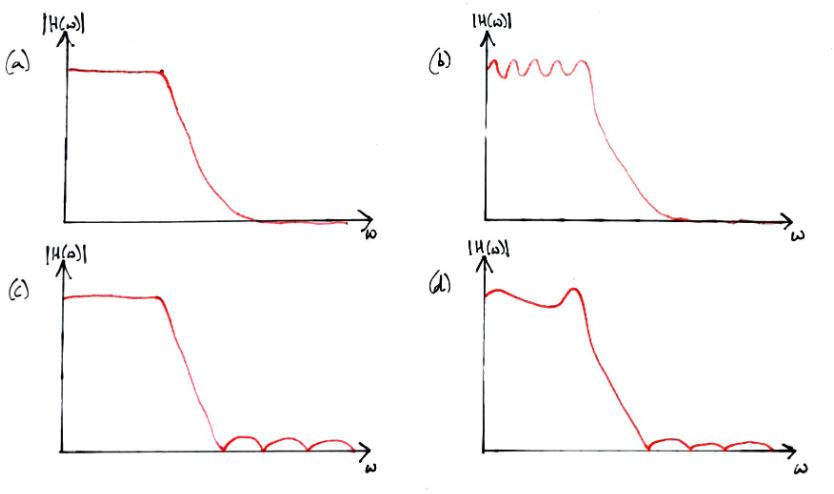
\includegraphics[width=\textwidth]{images/lecture_18_analog_filters.JPG}
  \caption{Four main types of analog filter. In pane (a), a Butterworth
    filter is shown which has frequency response as flat as possible in the
    pass-band (also referred to as a maximally flat magnitude filter). In
    pane (b), a Type I Chebyshev filter is shown, which has ripple in the
    pass-band but is flat in the stop-band. In pane (c), a Type II Chebyshev
    filter is shown, which has ripple in the stop-band but is flat in the
    pass-band. Finally, in pane (d) an elliptic filter is shown, which
    has equialised ripple in both the pass-band and stop-band (also
    referred to as a Cauer filter). The elliptic filter has a sharper cutoff
    than the others, at the expense of ripples on the whole bandwidth.
  }
  \label{fig::lecture_18_analog_filters}
\end{figure}
%
The problem is how to convert these continuous-time closed-form solution to
the digital time case. We suggest taking the continuous-time cases;
the impulse response $h_c(t)$ and its Laplace transform $H_c(s)$, and
sampling them at some rate to produce the discrete-time impulse response
$h[n]$ and its Z-transform $H(z)$. However, this is not trivial. For
$H_c(s)$ to be stable, its poles need to be contained to the left of the
imaginary axis, whereas for $H(z)$ to be stable, the poles need to be
contained within the unit circle. Performing this transformation requires
a complex conformal mapping, which is beyond the scope of these notes.\\
%
There are two main approaches to converting the continuous-time filters
to discrete time.

\subsubsection{Impulse Invariance}
%
Given some continuous-time impulse response $h_c(t)$, create a discrete-time
counterpart by sampling at rate $1/T$ and scale by $T$, such that
$h[n] = Th_c(nT)$. As we saw in the lecture on multirate processing, taking
this to the frequency domain with the DTFT yields a magnitude response which
is $2\pi$-periodic, and the cutoff frequency is scaled to $\omega_c T$.
Similarly, if we do not sample at a high enough rate, the periodic copies of
$|H(\omega)|$ might alias which is problematic since it fundamentally changes
the filter and will likely no longer be optimal in the digital world.

\subsubsection{The Bilinear Transformation}
%
This is much safer than impulse invariance. Consider the transformation
between the $s$ and $z$ domains,
%
\begin{displaymath}
  s = \frac{2}{T}\frac{z-1}{z+2} \quad\mathrm{and}\quad
  z = \frac{\frac{2}{T} + s}{\frac{2}{T} - s}
\end{displaymath}
%
Some examples of this \textbf{bilinear transformation} are presented in
Figure \ref{fig::lecture_18_bilinear_transform}.
%
\begin{figure}[!htb]
  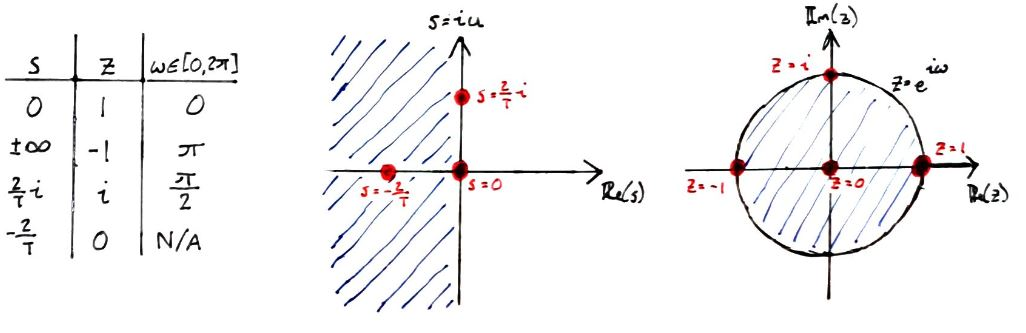
\includegraphics[width=\textwidth]{images/lecture_18_bilinear_transform.JPG}
  \caption{Examples of the bilinear transform between the $s$ and
    $z$ domains. Note that for the imaginary axis in the $s$ domain,
    $\im u$, $u$ is the continuous-time frequency with infinite range.
    The positive part of the $\im u$ axis wraps around to
    $0 \leq \omega \leq \pi$ in the $z$ domain, while the negative
    part of the $\im u$ axis wraps around to $-\pi \geq \omega \geq 0$
    in the $z$ domain. The hatched regions are those areas of the respective
    domains where the transforms don't converge; the left-half plane in
    the $s$ domain maps to the interior of the unit circle in the $z$ domain.
  }
  \label{fig::lecture_18_bilinear_transform}
\end{figure}
%
Consider the magnitude responses of the analog and digital filters in
Figure \ref{fig::lecture_18_prewarp}. These two filters are equivalent;
the cutoff frequency in the analog case transforms to some other
cutoff frequency in the digital case. Consequently, one has to take
steps to make sure the cutoff of the analog filter is chosen so as
to produce the desired cutoff in the digital filter.\\
%
The main idea is then to prewarp the desired digital filter cutoff
frequencies to the corresponding analog cutoffs using the $z\rightarrow s$
transformation. We then design an analog filter using this prewarped
cutoff frequency and warp back to a digital filter using the $s\rightarrow z$
transformation. If we comply with our filter specification in the
analog world (e.g. stop-band ripple, pass-band ripple, etc.), then
the digital filter will also comply to these specifications since
the bilinear transform only maps the domain; the responses will
stay the same -- a ripple in the $s$ domain will simply be squeezed
on stretched in the $z$ domain, its magnitude will not change.
%
\begin{figure}[!htb]
  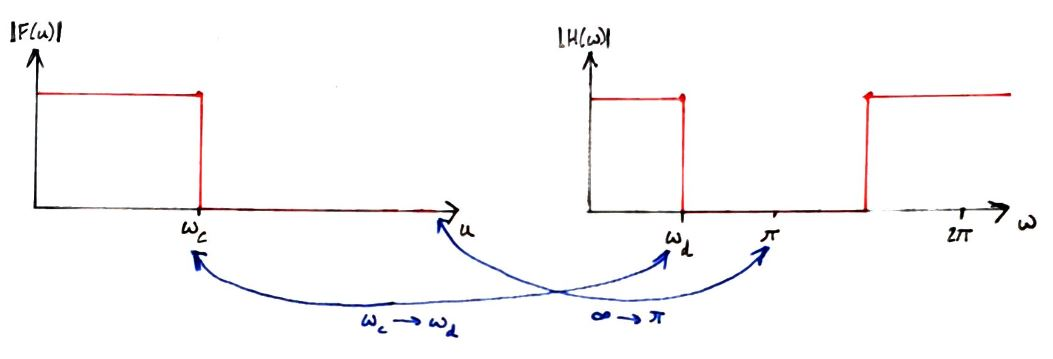
\includegraphics[width=\textwidth]{images/lecture_18_prewarp.JPG}
  \caption{The magnitude responses of an analog filter (left) and its
    digital counterpart (right). Under the
    bilinear transformation, $\omega_c\rightarrow\omega_d$. Also note
    that the mapping from $u=\infty$ to $z=\pi$ is shown.
  }
  \label{fig::lecture_18_prewarp}
\end{figure}
%
